

\begin{frame}
    \frametitle{Вкладка Общие}
    \begin{figure}[!ht]
           \begin{center}
               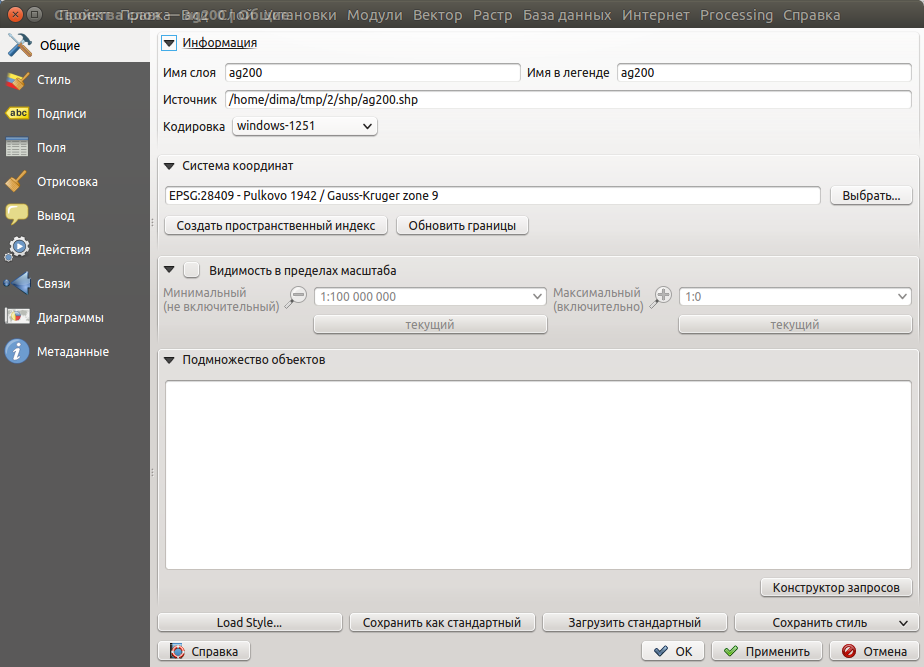
\includegraphics[width=0.95\columnwidth]{./practic/img/common.png}
           \end{center}
       \end{figure}
       Видимость в пределах масштаба.
\end{frame}

\begin{frame}
    \frametitle{Вкладка Стиль}
    \begin{figure}[!ht]
           \begin{center}
               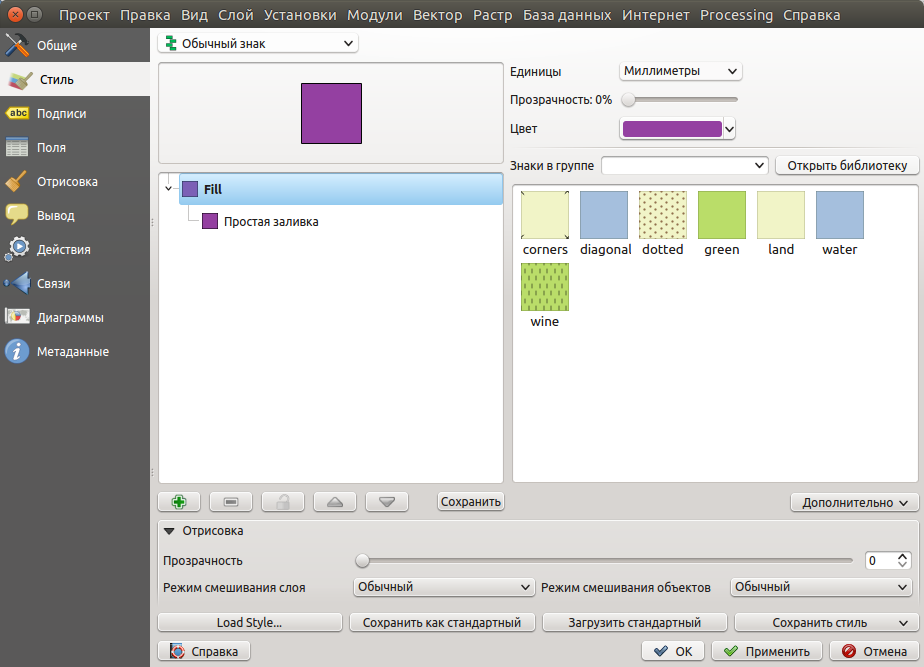
\includegraphics[width=0.95\columnwidth]{./practic/img/style.png}
           \end{center}
       \end{figure}
       Основная вкладка по стилям.
\end{frame}

\begin{frame}[allowframebreaks]
    \frametitle{Вкладка Стиль: градуировка знака}
    \begin{itemize}
        \item Обычный знак
        \item Уникальные значения (номинальные)
        \item Градуированный знак (порядковые)
        \item Правила (фильтр по значениям и видимость в пределах масштаба)
        \item Точки со смещением
        \item Инвертированные полигоны (фон -- цветом полигона, полигон -- белым)
    \end{itemize}
\end{frame}

\begin{frame}[allowframebreaks]
    \frametitle{Вкладка Стиль: режим смешения слоев}
    Пиксели, принадлежащие текущему слою и нижележащим слоям, смешиваются в соответствии с заданным алгоритмом.
    \begin{itemize}
        \item Normal: Цвета не смешиваются.
        \item Lighten: Выбирается самый светлый из всех нижележащих слоев.
        \item Screen: Светлые пиксели низлежащих слоев отрисовываются в текущем, а темные нет. (Используется для копирования текстур с других слоев).
        \item Dodge: Осветление низлежащих пикселей до уровня яркости пикселя текущего слоя.
        \item Addition: Суммирование яркостей пикселей слоев. Если сумма больше 1, получаем белый цвет.
        \item Darken: Выбирается самый темый пиксель.
        \item Multiply: Умножаются яркости пикселей.
        \item Burn: Темные пиксели верхнего слоя затемняют пиксели низлежащего слоя.
        \item Overlay: Комбинация Multiply и Screen.
        \item Soft light: Комбинация Burn и Dodge.
        \item Difference: Вычитается из вернего пикселя пиксель нижнего пиксель (или наоборот --- чтобы не уйти в минус).
        \item Subtract: Как и ранее, из верхнего вычитается минимум, но отрицательные значения заменяются нулем.
    \end{itemize}
\end{frame}

\begin{frame}
    \frametitle{Вкладка Подписи}
    \begin{figure}[!ht]
           \begin{center}
               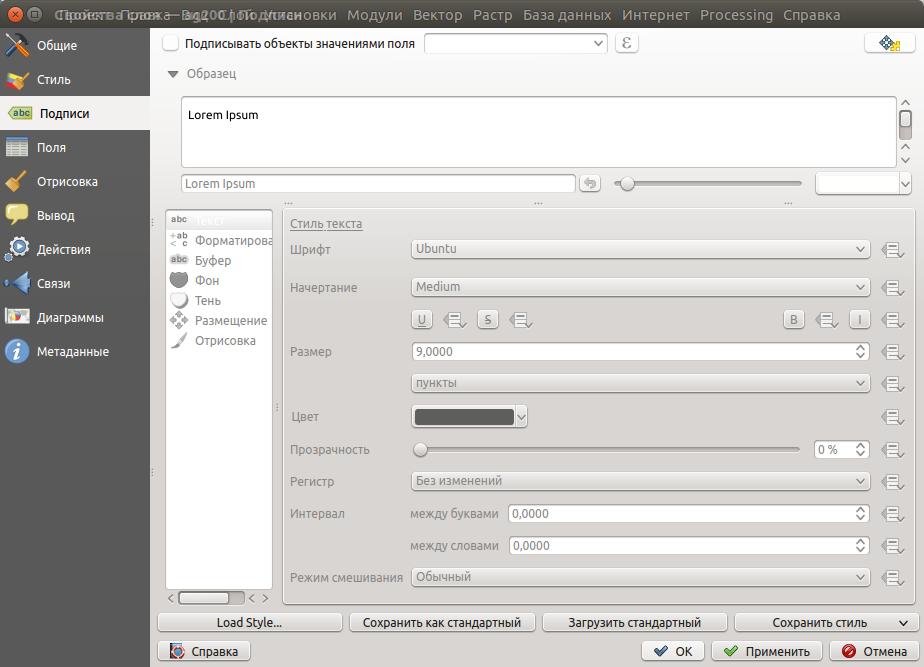
\includegraphics[width=0.95\columnwidth]{./practic/img/labels.png}
           \end{center}
       \end{figure}
\end{frame}

\begin{frame}
    \frametitle{Вкладка Вывод}
    \begin{figure}[!ht]
           \begin{center}
               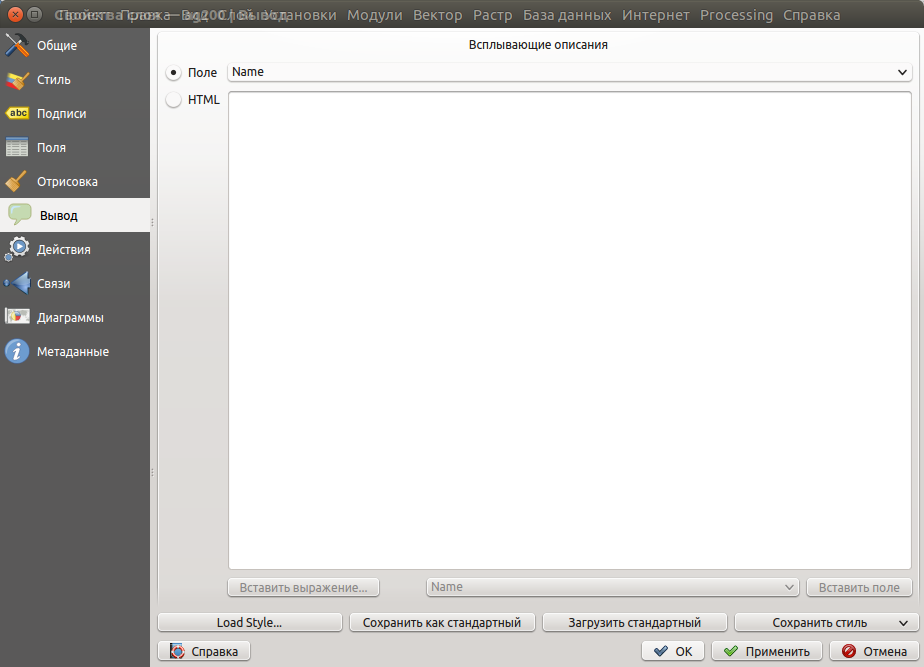
\includegraphics[width=0.95\columnwidth]{./practic/img/hints.png}
           \end{center}
       \end{figure}
\end{frame}


\begin{frame}
    \frametitle{Вкладка Диаграммы}
    \begin{figure}[!ht]
           \begin{center}
               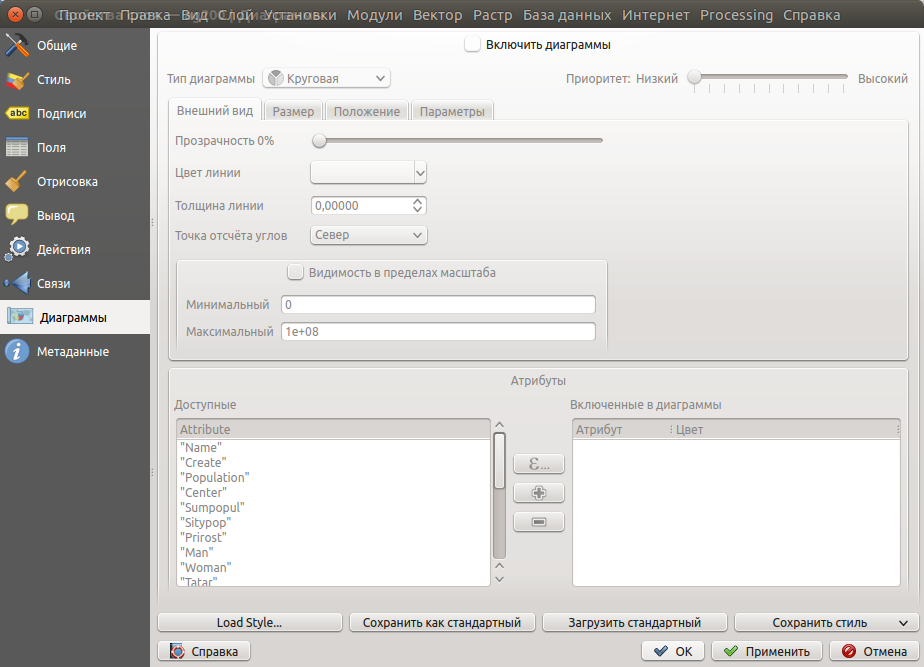
\includegraphics[width=0.95\columnwidth]{./practic/img/diagrams.png}
           \end{center}
       \end{figure}
\end{frame}

\begin{frame}
    \frametitle{Задание}
    Масштаб 1: в этом масштабе в окне видна вся карта. Видны общие границы республики и границы районов с названиями, административные центры в виде точки. На карту выводятся подписи районов.

    Масштаб 2: в этом масштабе в окне видна карта выбранного района с его названием. При достижении данного масштаба видны дороги и реки, административные центры нанесены на карту в виде точки.

    Масштаб 3: в этом масштабе ваш район достигает увеличения в 2 раза  (масштаб 3 крупнее масштаба 2 в 2 раза), при этом должны быть видны все слои, а также отображаться названия населенных пунктов. Административный центр не должен отображаться точкой.

    Масштаб 4: в этом масштабе района достигает увеличения в 4 раза. В этом масштабе на карте видны все слои, названия населенных пунктов и рек. Название района не отображается.

    Масштаб 5: в этом масштабе карта района достигает увеличения в 8 раз. Видны все слои и названия всех объектов.
\end{frame}


\begin{frame}
    \frametitle{Кодировка типов автодорог}
    \begin{description}
        \item[61210000] Автомагистрали (автострады)
        \item[61220000] Автодороги с улучшенным покрытием
        \item[61230000] Автодороги с покрытием (шоссе)
        \item[61240000] Дороги с твердым покрытием
        \item[61310000] Автодороги без покрытия
        \item[61320000] Грунтовые проселочные дороги
        \item[61330000] Полевые и лесные дороги
        \item[61500000] Автодороги с дерев. покрытием
        \item[61940000] Труднопроезжие участки дорог
    \end{description}
\end{frame}
